\documentclass[french, a4paper, 12pt]{article}% si la table des matieres est petite
\usepackage{blindtext}
\usepackage[T1]{fontenc}
\usepackage[utf8]{inputenc}
\usepackage[french]{babel}
\usepackage{graphicx,color, caption}
\usepackage{epsfig}
\usepackage{fancyhdr}
\usepackage{textcomp}
\usepackage{listings}		% pour incorporer des sources
\usepackage[francais]{layout}	% pour obtenir le layout
\usepackage{fullpage}		% pour obtenir le layout
\usepackage{makeidx}		% pour créer une table d'index
\usepackage{shadow}		% pour faire des encadrements
\usepackage{setspace}
\usepackage{fancyhdr}
\usepackage{xcolor}
\usepackage{enumitem}
\usepackage{tcolorbox,listings}
\usepackage{fullpage}
\usepackage{color}
\usepackage{multicol} %positionner plusieurs images sur une ligne
\usepackage{lipsum}
\usepackage{mwe}
\usepackage{graphicx} %nécessaire pour les imafes
\usepackage{float} % ici: H option pour float 
\usepackage{subcaption} % charge le package caption


% Modification des marges ------------------------------
\oddsidemargin -4mm 	% Marge de gauche -4mm
\textwidth 17cm 	% Largeur de gauche = 17cm
\textheight 22cm 	% Hauteur du texte = 22cm
\parindent 0cm		% Pas d'indentation de paragraphe
% -----------------------------------------------------

\pagestyle{fancy}
\pdfminorversion=7
\headsep = 30pt

% Modification du cadre des codes source ------------------------------
\definecolor{darkWhite}{rgb}{0.94,0.94,0.94} 
\lstset{
    backgroundcolor=\color{darkWhite},
    breakatwhitespace=false,
    breaklines=true,
    captionpos=b,
    commentstyle=\color{violet},
    deletekeywords={...},
    escapeinside={\%*}{*)},
    extendedchars=true,
    keepspaces=true,
    keywordstyle=\color{blue},
    language=C,
    morekeywords={*,...},
    showspaces=false,
    showstringspaces=false,
    showtabs=false,
    stepnumber=1,
    stringstyle=\color{gray},
    tabsize=4,
    title=\lstname,
    basicstyle=\footnotesize,
    numbers=left,
    stepnumber=1,
    showstringspaces=false,
    tabsize=1,
    breaklines=true,
    breakatwhitespace=false,
}
 
\lstdefinestyle{frameStyle}{
    basicstyle=\footnotesize,
    numbers=left,
    numbersep=20pt,
    numberstyle=\tiny\color{black}
}
 
\tcbuselibrary{listings,skins,breakable}
 
\newtcblisting{customFrame}{
    arc=0mm,
    top=0mm,
    bottom=0mm,
    left=3mm,
    right=0mm,
    width=\textwidth,
    listing only,
    listing options={style=frameStyle},
    breakable
}

\begin{document}

% Page de garde --------------------------------------
\begin{titlepage}
    \begin{center}
        \vspace*{0.5cm}
            
        \Huge
        \textbf{Stéganographie : Bitmap et GIF}
            
        \vspace{0.5cm}
        \LARGE
           
        \vspace{0.5cm}
            
        \textbf{Foud Hind et Patti Philippe}
            
        \vfill
        Projet de stéganographie sur fichier image Bitmap et GIF  
        réalisé pour le cours de SYSG5
            
        \vspace{4cm}
            
        
\includegraphics[width=0.3\textwidth]{esi.eps}
    \end{center}
\end{titlepage}


% Numérotation et table des matières -----------------
\setcounter{tocdepth}{3}    % fixe la profondeur de la table des matières
\setcounter{secnumdepth}{-1} % fixe la profondeur de la numérotation des sections et paragraph

\lhead{}
\rhead{}
\doublespacing
\newpage
\tableofcontents
\singlespacing

% Titres sur  chaque page -----------------------------

\rhead{Stéganographie - Bitmap / GIF}
\lfoot{\copyright{Foud Hind, Patti Philippe}}
\cfoot{ } % Bas centre - obligatoire !
\rfoot{\thepage} % Bas droite
\renewcommand{\headrulewidth}{0.3pt} 
\renewcommand{\footrulewidth}{0.3pt} 

% Inclusion des textes
\section{Introduction}
L'objectif du projet est d'implémenter un programme illustrant le concept de sécurité suivant : la stéganographie.\\

Abordée du point de vue du cours de système, elle nous permet d'approfondir nos connaissances sur l'utilisation de la mémoire
pour stocker des informations.\\

Il est évident que pour mener à bien un projet de cette envergure, d'autres compétences nous ont été nécessaires
telles que l'apprentissage approfondi du langage C, notamment pour réaliser des opérations de manipulation de bits.
Nous avons également eu besoin d'apprendre en détails les structures de fichier bitmap et GIF, pour décider de la meilleure technique à
utiliser afin d'y cacher des messages.\\

Dans ce rapport, nous passerons en revue l'organisation du projet, le choix pour chaque format et la technique utilisée. 
Nous fournirons aussi un guide pratique pour utiliser les exécutables. 

\vspace{1.5cm}


\newpage
\section{Organisation du projet}
La structure de notre projet s'organise essentiellement en quatre répertoires dont voici le détail :\\ 

\begin{itemize}
    \item \textbf{dist :} contient les exécutables du programme dans un dossier bmp et gif respectifs.
    \item \textbf{rapport :} contient le rapport en format tex et pdf, les fichiers qui serviront à construire celui-ci 
    ainsi que le makefile qui le lancera. On pourra également y trouver le document pdf de la présentation.
    \item \textbf{rsc :} contient les ressources qui servent d'input au programme [bitmap et gif] ainsi que les outputs 
    qui seront produits dans un dossier bmp et 
    gif respectifs.
    \item \textbf{src :} contient les sources du programme dans un dossier bmp et gif respectifs\\
\end{itemize}
On peut également trouver à la racine, un makefile général qui automatise le lancement du programme ainsi qu'un fichier README.

\vspace{1.5cm}
\section{Guide pratique}
\lstinputlisting[language=make, firstline=1, lastline=18]{../makefile}

\newpage
\section{Stéganographie : Définition}
La stéganographie est l'art de la dissimulation : son objet est de faire passer inaperçu des données dans d'autres données. 
Elle se distingue de la cryptographie, « art du secret », qui cherche à rendre un message inintelligible à autre que qui-de-droit.\\
Les fichiers peuvent être de type divers : fichiers image, audio, html, vidéos etc.\\
Parmi les scénarios de tests envisagés, nous avons tenté de cacher :\\

\begin{itemize}[label=$\diamond$, font=\LARGE \color{black}]
    \item un \textbf{texte} (.txt, .pdf) dans une \textbf{image} (.bmp/.gif)
    \item une \textbf{image} (.bmp, .gif) dans une \textbf{image} (.bmp/.gif)
    \item une \textbf{vidéo} (.mp4) dans une \textbf{image} (.bmp/.gif)\\
\end{itemize}


Il est évident que pour que cela soit possible, des conditions sont à poser.
Il faudra bien sûr que le fichier à cacher soit plus petit que le fichier objet. Il faudra aussi peauffiner les conditions de 
faisabilité qui sont fortement dépendantes du type de fichier et veiller à respecter la règle d'or : le dissimuler à tout prix.
Cela signifie qu'il faudra limiter au maximum l'impact sur le fichier dans lequel on aura caché des données sinon ce serait contraire
au principe de stéganographie.


\newpage
\section{Least Significant Bit (L.S.B.)}
Pour coder/décoder un message, nous employons la technique du Least Significant Bit (LSB). \\
Comme vous le voyez sur le schéma ci-dessous [Schéma général], cette technique consiste à se focaliser sur le bit le moins 
important d'un byte appelé le bit de poids faible.
Pour coder le message, il suffit de lire un byte à cacher et de l'encoder dans le bit de poids faible d'un byte choisi.
Pour décoder le message, il suffit de lire le bit de poids faible de ces bytes 'élus' et de reformer un message compréhensible.\\\\


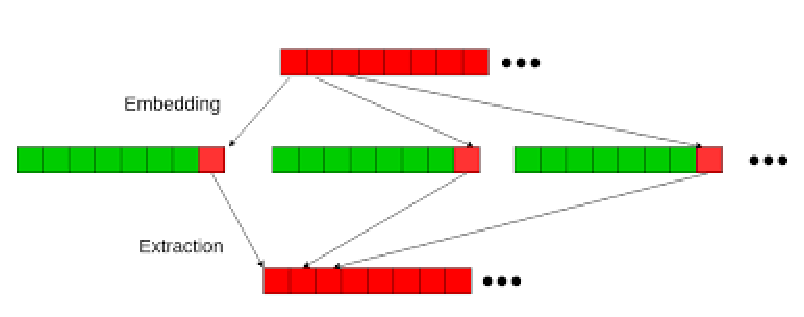
\includegraphics[width=12cm]{lsb.eps}\\\\


C'est cette logique que nous nous sommes employés à suivre dans le cas de traitement sur ces deux formats de fichiers image.
Ainsi, la technique est la même mais certains choix se sont imposés de part les différences entre les deux structures de ces 
fichiers image. Ces choix portent notamment sur 'l'élection' des bytes dans lesquels nous allons cacher l'information.
En effet, pour que le message ait le plus petit impact possible sur le fichier image, il faut employer des bytes qui peuvent
perdre un bit d'information sans que cela ne se remarque.
Par exemple, pour une couleur codée en rgb, le changement du dernier bit a un impact très faible, quasi invisible à l'oeil nu.
Il est donc adéquat pour y dissimuler des données.\\\\


\subsection{Encodage : extrait de code source concernant la manipulation des LSB}
\lstinputlisting[language=c, firstline=57, lastline=72]{../src/utils/bmp.c}

\subsection{Décodage : extrait de code source concernant la manipulation des LSB}
\lstinputlisting[language=c, firstline=91, lastline=101]{../src/utils/bmp.c}

\vspace{1.5cm}


\section{Bitmap}

\subsection{Aperçu du Bitmap}
Le format BITMAP aussi appelé DIB (Device Independent Bitmap) a été conçu par Windows corporation pour pouvoir échanger des images entre devices sans avoir à se soucier de la logique de ceux-ci.
Ces images ont des extensions .bmp ou encore .dib.\\
Une image bitmap est un format de fichier généralement non compressé. Cela signifie que chaque pixel possède sa représentation sous forme d'une série de bits.
Les bitmaps n'ont aucune perte de données et sont donc généralement plus lourds.
On peut opposer leur structure à celle d'une image PNG, JPEG ou encore GIF, qui utilisent la compression pour regrouper des pixels similaires.\\
Les headers des bitmaps peuvent employer plusieurs versions. Ces versions donnent plus ou moins de métadonnées sur le bitmap. 
Le BITMAPINFOHEADER est une des versions les plus simples et rétrocompatible. 
Actuellement, il existe des versions plus complètes, tels que le BITMAPV4HEADER ou BITMAPV5HEADER.\\
La structure du format BITMAP est connue et disponible en ligne. En voici un schéma, utilisant le BITMAPINFOHEADER :\\

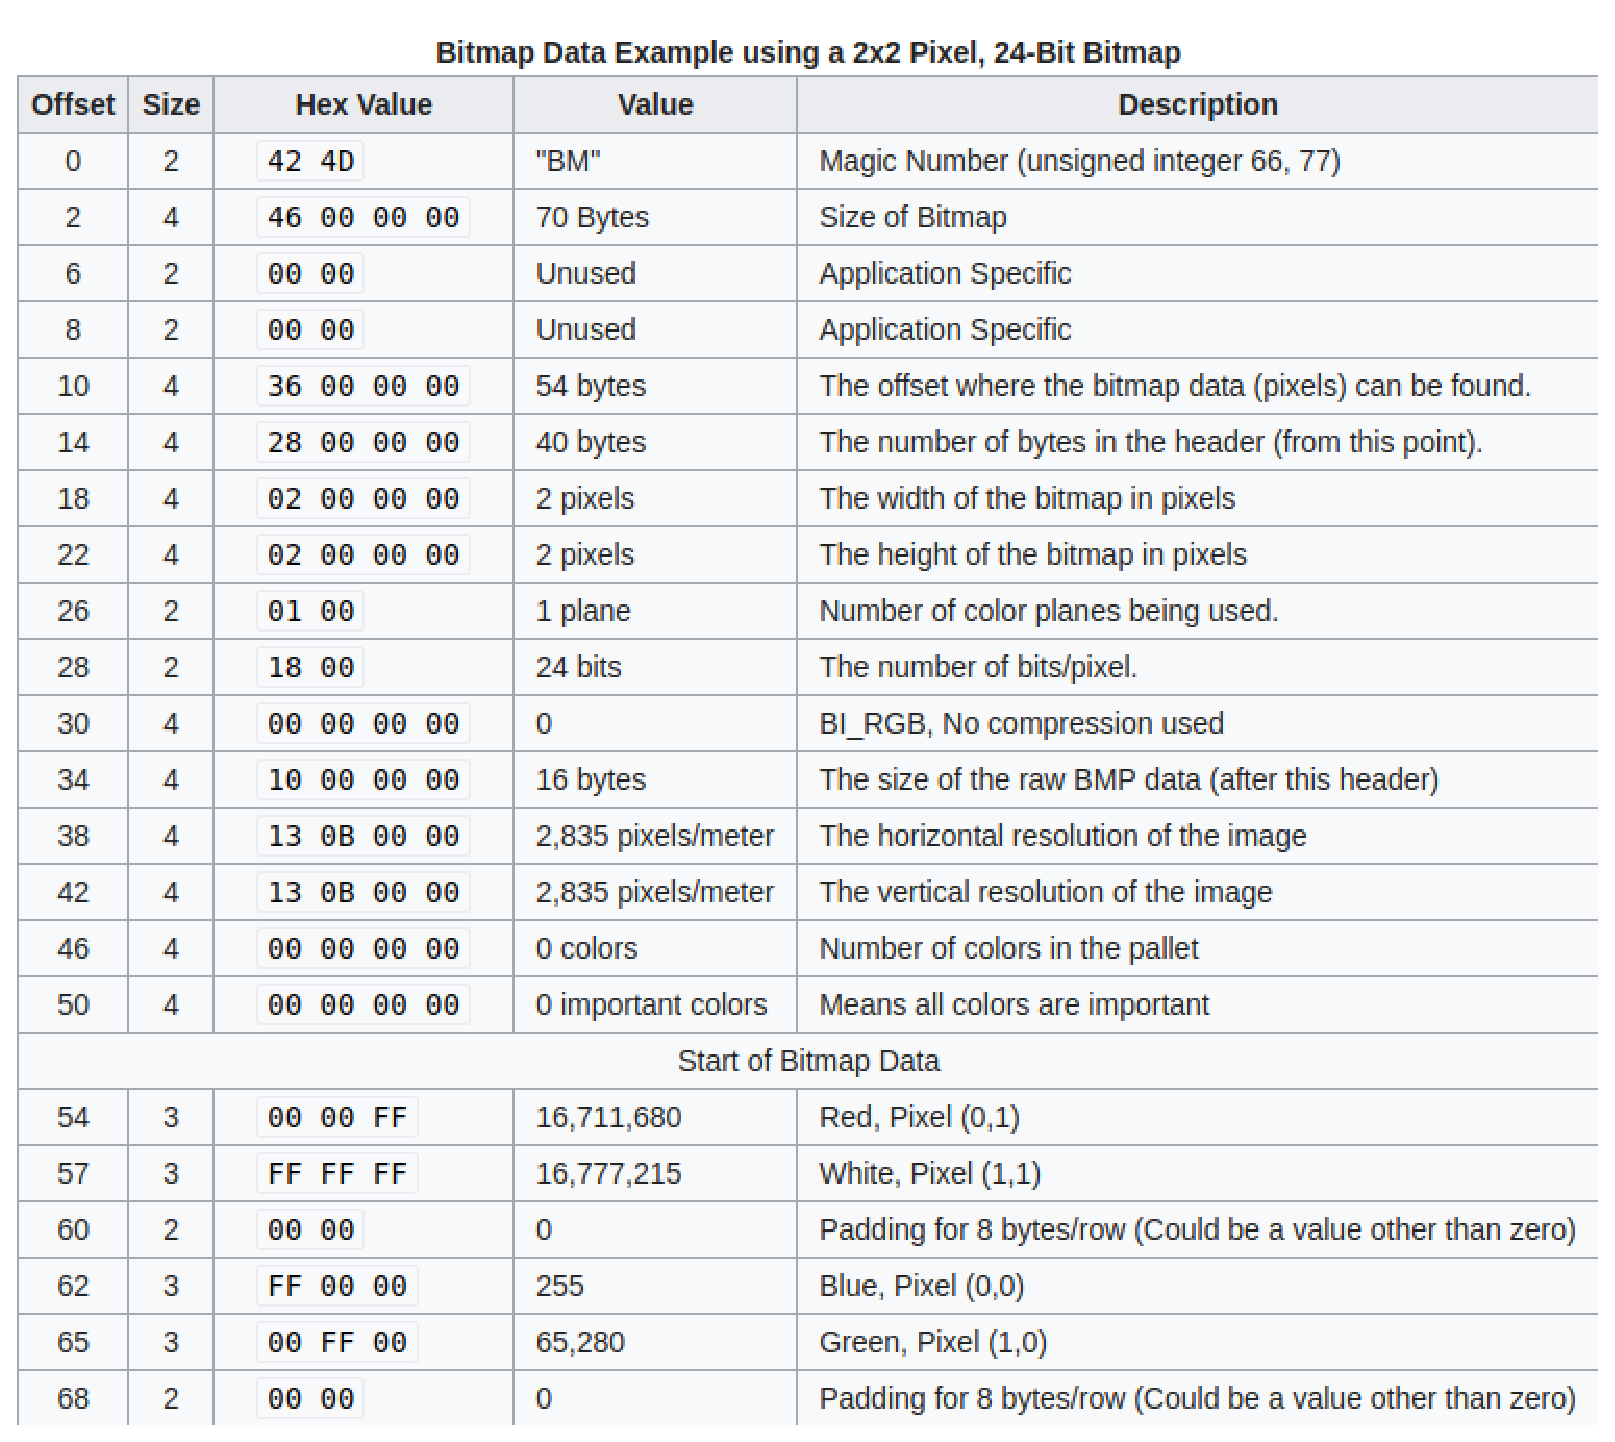
\includegraphics[width=14cm]{bitmap_structure.eps}\\\\

\subsection{Application du LSB}
Nous cachons les données dans les bytes décrivant les couleurs de l'image source, juste après le header.
Les modifications étant faites sur des couleurs, l'image est peu altérée. Les modifications sont invisibles à l'oeil humain.
De plus, ce fichier n'utilisant généralement pas d'algorithme de compression, on ne doit pas se soucier de perte de données, 
ce qui impacteraient le décodage d'une image dans laquelle on aurait caché des données.

\vspace{1.5cm}

\begin{figure}[H]
    \centering
    \subcaptionbox{Bitmap source}{
\includegraphics[width=0.45\textwidth]{splash_color_src.eps}}%
    \hfill
    \subcaptionbox{Bitmap dest }{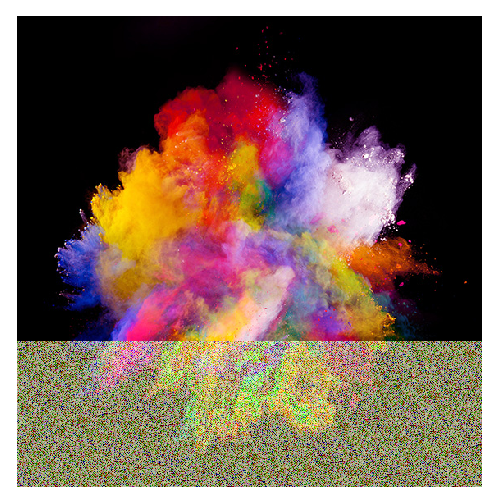
\includegraphics[width=0.45\textwidth]{splash_color_dest.eps}}%
    \caption{Encodage d'un fichier texte dans un bitmap}
\end{figure} 
\section {GIF}

\subsection {Pourquoi le GIF?}
Le format GIF permet de stocker plusieurs images dans un fichier. 
Ceci permet de créer des diaporamas, voire des animations si les images sont affichées à un rythme suffisamment soutenu. 
Chaque image d'une animation peut avoir sa propre palette.
Le GIF est un format très utilisé, particulièrement sur les réseaux sociaux. 
Ce projet peut donc intéressé pas mal de gens. \\\\

La structure du format GIF est connue et disponible en ligne. En voici un schéma : \\\\

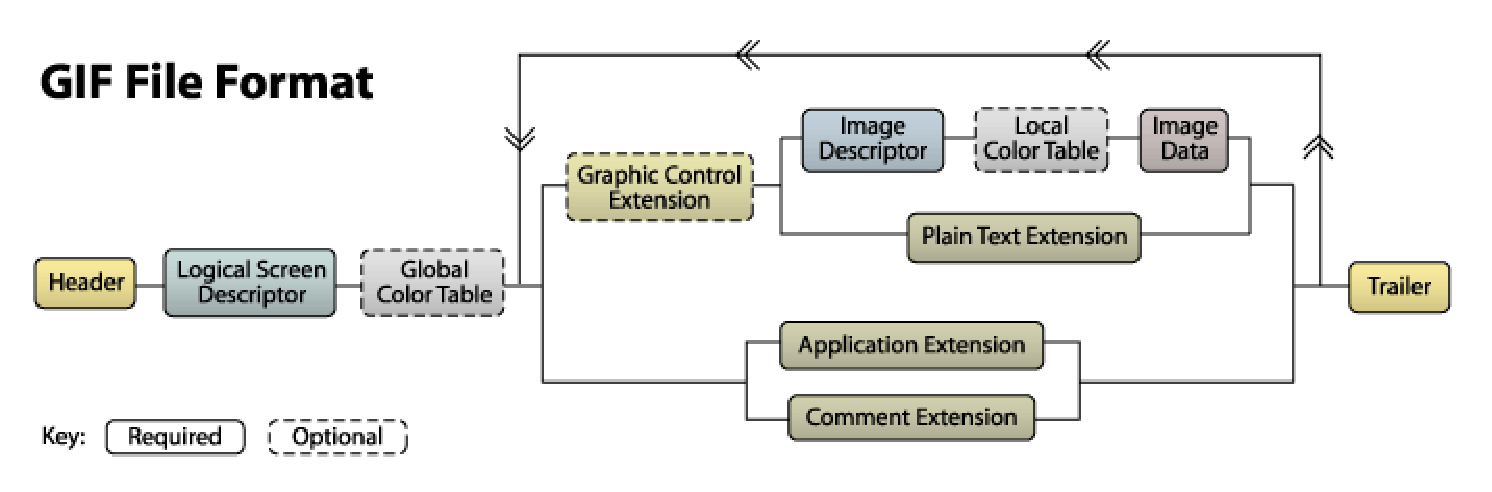
\includegraphics[width=15cm]{gif_structure.eps}


\subsection {Application du LSB}
Nous avons choisi de cacher des informations dans les couleurs qui se trouvent dans les Local Color Table. 
Cette section facultative peut revenir devant chaque bloc image data. Si cette section n'existe pas, nous la rajoutons.\\\\

Il est possible de calculer la taille maximale du message cachée à l'avance : 
en comptant le nombre de bloc image data et en le multipliant par le nombre de byte dans la Global Color Table.


\subsection {Avancement}
\subsubsection {Lecture}
Le programme peut déja lire un gif en entier, section par section. 
Les tailles des sections sont indiquées à des endroits différents par sections. 
La lecture se fait donc différemment en fonction de la section.\\\\

De plus, on peut déja savoir le nombre maximal de Local Color Table pour le fichier modifié.

\subsubsection {Lecture}
Le programme réécrit le gif dans un nouveau fichier, en insérant des Local Color Table, identique à la Global Color Table. 
Ceci permettra d'y insérer un message. 
L'insertion du message devrait être évidente, vue qu'elle sera presque identique à la stéganographie dans un fichier bitmap.\\\\

Il y a toutefois encore un bug dans la réécriture du fichier gif, probablement à l'écriture des nouvelles Local Color Table.
%\section {Conclusion}
\printindex			% Impression de la table des index
\end{document}
